\documentclass[a4paper]{article}

\usepackage[english]{babel}
\usepackage[utf8x]{inputenc}
\usepackage{amsmath}
\usepackage{graphicx}
\usepackage[colorinlistoftodos]{todonotes}
\usepackage{fullpage}
\usepackage{amsfonts}
\usepackage{hyperref}
\usepackage{url}
\usepackage{pdfpages}

\title{Report of Project: Forward-Planning Agent}
\author{Israel G. de Oliveira}
\date{January 8, 2019}
\begin{document}
\maketitle

\section{Introduction}
This report is about the building a Forward-Planning Agent, project part from Artificial Intelligence Nanodegree \cite{githubUdacityAIND}. The objective is implement functions to able a agent to solve planning problems based on symbolic logic and classical search (progression search), doing experiments with different search algorithms and heuristics \cite{githubUdacityAINDProj2}. This project is based on book Artificial intelligence: a modern approach \cite{russell2009artificial}.

\subsection{Planning Problems}

The planning problems used is based on the example Air Cargo Problem, 10.1.1 from \cite{russell2009artificial}, with four sized variants \cite{githubUdacityAINDProj2}, in according with the Table \ref{airps}. 

\begin{table}[htpb]
   \caption{ Air Cargo Problems}
    \label{tab:cronograma}
    \centering
        \begin{tabular}{ c | c | c | c}
           Problem nº & Planes & Cargos & Airports \\\hline
           1          & 2      & 2      & 2 \\
           2          & 3      & 3      & 3 \\
           3          & 2      & 4      & 4 \\
           4          & 2      & 5      & 4 \\\hline
        \end{tabular}
        \label{airps}
\end{table}

One way to solve this problems is use a graph representation connecting all logic literals and possible actions. With a graph, it is possible to use a search algorithm to find a solution \cite{russell2009artificial}. Not only, for some search algorithms, it is possible to use a heuristic method to estimate the cost for each node (in graph), in some cases, improving the finding for a solution (less time expending on searching).

\subsection{Search Algorithms}

The search algorithms proposed to use are Breadth First Search (BFS), Depth First Graph Search (DFS), Uniform Cost Search (UCS), Greedy Best First Graph Search (GBFGS) and A* Search \cite{githubUdacityAINDProj2}. All this algorithm is already implemented with the framework provided by Udacity, available in \cite{githubUdacityAINDProj2}.

BFS is a instance of the tree search with FIFO (First In, First Out) queue. This algorithm is complete (completeness aspect). The solution is not necessarily optimal: because when a objective node is found at a (depth) level $d$ it is not necessarily the best objective node. The total new nodes is $O(b^d)$ with $b$ successors. 

Considering the same step cost 1 for all nodes, we have the BFS. For achieve the UCS, we do a extended version considering a step cost function $g(n)$, for a $n$-node, then is possible to achieve a optimal solution. Basically, expanding the node with the lowest cost. There are more two differences from BFS: the first is when the objective node is selected for expansion, and not when it is generated, the second is the additional test, to find a possible better path for a objective node. The solution is, generally, optimal. The completeness is not guaranteed, because the number of steps in a path is not relevant, only your cost. If there is a infinity sequence of actions with zero cost (like \emph{NoOp} actions), the search is not finite. The complexity is $O(b^{1+ \lfloor C^*/\epsilon \rfloor})$, with the optimal solution cost $C^*$ and lowest action cost $\epsilon$. If all actions have the same cost, the complexity is $O(b^{d+1})$. In this case, UCS expands all nodes of the same depth, even though the solution has already been found (at this depth).

DFS is a instance of graph (tree) search with a LIFO (Last in, First out) queue. This algorithm search the nodes without repetition (and redundant paths). The graph version is finite, but the tree not. The complexity is $O(b^m)$, with $m$ the max depth of any node. Observe that $m$ can be infinite, even greater than the state space. The advantage in use this algorithm is the space complexity: $O(bm)$, using much less memory. As the algorithm returns the solution when it finds the first objective node, ignoring other possible best nodes, the solution is not, necessarily, optimal.

GBFGS try expand the node nearest from the objective, with the idea of finding the solution quickly. In this way, only the heuristic function is considered. Even with a finite states, the completeness is not guaranteed. The complexity is $O(b^{\epsilon d})$, with $m$ the max depth of state-space. The solution is not, necessarily, optimal because the greedy aspect, trying always get closer to node objective, choosing paths larger than possible others with intermediate nodes further from the node objective.

A* (so-called \emph{a-star}), differing from UCS only by the cost function, considering plus a heuristic cost function $h(n)$ from a $n$-node to the objective node, resulting the cost function $f(n) = g(n) + h(n)$. Satisfying certain conditions, the completeness and the optimal solution is guaranteed. The complexity is $O(b^{\epsilon d})$, where the $d$ the detph solution and $\epsilon$ is the heuristic error. Basically, Basically, the performance depends on the quality of the heuristics used.

\subsection{Heuristics}

Basically, with a good heuristic is possible to achieve a better performance using a search algorithm. All descriptions below are copied from the \cite{githubUdacityAINDProj2}.
\begin{itemize}
    \item \textbf{LevelCost}: "The level cost is a helper function used by MaxLevel and LevelSum. The level cost of a goal is equal to the level number of the first literal layer in the planning graph where the goal literal appears."
    \item \textbf{MaxLevel}: "The max-level heuristic simply takes the maximum level cost of any of the goals; this is admissible, but not necessarily accurate" \cite{russell2009artificial}.
    \item \textbf{LevelSum}: "The level sum heuristic, following the subgoal independence assumption, returns the sum of the level costs of the goals; this can be inadmissible but works well in practice for problems that are largely decomposable" \cite{russell2009artificial}.
    \item \textbf{SetLevel}: "The set-level heuristic finds the level at which all the literals in the conjunctive goal appear in the planning graph without any pair of them being mutually exclusive" \cite{russell2009artificial}.
\end{itemize}

\section{Search Algorithms Results}

For all experiments, was used a Intel(R) Xeon(R) CPU E3-1241 v3 @ 3.50GHz, on Ubuntu 18.04.1 LTS, Linux kernel 4.15.0-43-generic and PyPy 6.0.0 with GCC 4.8.2. All results, without the \path{my_planning_graph.py}, is available in \cite{githubYsraellAIND}. All analysis of the results is based on \cite{russell2009artificial}.

In table \ref{airps1}, for problem 1, only DFGS not achieve the optimal solution. In table \ref{airps2}, problem 2, A*, UCS and BFS achieved the optimal solution. 

\begin{table}[htpb]
    \caption{Air Cargo Problem 1}
    \centering
    \begin{tabular}{ l | c }
    Search Method & Plan length \\ \hline 
BFS & 9 \\
DFGS & 619 \\
UCS & 9 \\
GBFGS w. Unmet Goals & 9 \\
GBFGS w. LevelSum & 9 \\
GBFGS w. MaxLevel & 9 \\
GBFGS w. SetLevel & 9 \\
A* w. Unmet Goals & 9 \\
A* w. LevelSum & 9 \\
A* w. MaxLevel & 9 \\
A* w. SetLevel & 9
\end{tabular}
    \label{airps1}
    \end{table}

    
\begin{table}[htpb]
    \caption{Air Cargo Problem 2}
    \centering
    \begin{tabular}{ l | c }
    Search Method & Plan length \\ \hline 
BFS & 14 \\
DFGS & 24132 \\
UCS & 14 \\
GBFGS w. Unmet Goals & 18 \\
GBFGS w. LevelSum & 17 \\
GBFGS w. MaxLevel & 17 \\
GBFGS w. SetLevel & 23 \\
A* w. Unmet Goals & 14 \\
A* w. LevelSum & 15 \\
A* w. MaxLevel & 14 \\
A* w. SetLevel & 14
\end{tabular}
    \label{airps2}
    \end{table}

For the other problems 3 and 4, it is similar to the other two problems. A*, UCS and BFS achieved the optimal solution, save some differences between heuristics. 
    
\begin{table}[htpb]
    \caption{Air Cargo Problem 3}
    \centering
    \begin{tabular}{ l | c }
    Search Method & Plan length \\ \hline 
BFS & 6 \\
DFGS & 20 \\
UCS & 6 \\
GBFGS w. Unmet Goals & 6 \\
GBFGS w. LevelSum & 6 \\
GBFGS w. MaxLevel & 6 \\
GBFGS w. SetLevel & 6 \\
A* w. Unmet Goals & 6 \\
A* w. LevelSum & 6 \\
A* w. MaxLevel & 6 \\
A* w. SetLevel & 6
\end{tabular}
    \label{airps3}
    \end{table}

    
\begin{table}[htpb]
    \caption{Air Cargo Problem 4}
    \centering
    \begin{tabular}{ l | c }
    Search Method & Plan length \\ \hline 
BFS & 12 \\
DFGS & 392 \\
UCS & 12 \\
GBFGS w. Unmet Goals & 15 \\
GBFGS w. LevelSum & 14 \\
GBFGS w. MaxLevel & 13 \\
GBFGS w. SetLevel & 17 \\
A* w. Unmet Goals & 12 \\
A* w. LevelSum & 12 \\
A* w. MaxLevel & 12 \\
A* w. SetLevel & 12
\end{tabular}
    \label{airps4}
    \end{table}
    
\newpage

%\subsection{BFS: Breadth First Search}
%\subsection{DFS: Depth First Graph Search}
%\subsection{UCS: Uniform Cost Search}
%\subsection{GBFGS: Greedy Best First Graph Search}
%\subsubsection{Unmet Goals Heuristic}
%\subsubsection{PG Level Sum Heuristic}
%\subsubsection{PG Max-Level Heuristic}
%\subsubsection{PG Set-Level Heuristic}
%\subsection{A*: A-Star Search}
%\subsubsection{Unmet Goals Heuristic}
%\subsubsection{PG Level Sum Heuristic}
%\subsubsection{PG Max-Level Heuristic}
%\subsubsection{PG Set-Level Heuristic}

In Figure \ref{figsm234} we observe what is expected: the UCS and BFS expand more than DFS. In problem 1 and 2, the behavior is practically equal, differing drastically in problem 3 and 4. The graph representing the problem 3 is more depth than problem 2 (or problem 2 is more wide). That explain how much larger is the plan length given by DFS for all problems and why the time consumption is lowest in p. 3 in relation to p. 2. Other thing that is possible to infer from Figure \ref{figsm231}, is the larger time taken with p. 4, because the graph if not only deeper then others, but is larger (wide). The little difference between UCS and BFS may be explain because both search the objective trying find the shortest path, for BFS, and the cheaper path, for UCS, but UCS takes a bit more time (and expansion) because the search continuous trying to find a cheaper path (than reached).

\begin{figure}[htpb]
\begin{center}
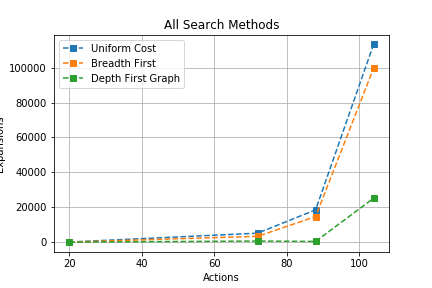
\includegraphics[width=1\columnwidth]{fig/results_sm234.png}
\end{center}
\caption{Search algorithms without heuristic.}
\label{figsm234}
\end{figure}
    
\begin{figure}[htpb]
\begin{center}
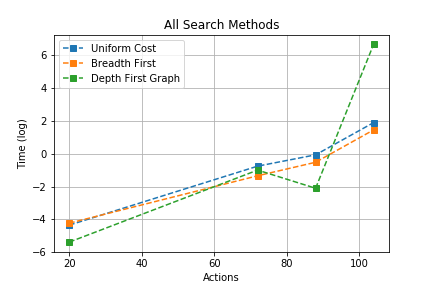
\includegraphics[width=1\columnwidth]{fig/results_sm231.png}
\end{center}
\caption{Search algorithms without heuristic.}
\label{figsm231}
\end{figure}

%\subsection{Greedy Best First Graph Search}


        
GBFGS algorithm takes more time, as seen on Figure \ref{fig131}, than all others, bot less expansions than UCS and BFS, Figure \ref{fig134}. For p. 1 and 3, the solution is optimal, but for p. 2 and 4, is not optimal, some solutions is near optimal. This results is expected because, even with a good heuristic, the search try expand to node closest to objective, doing something like a penalization of the other nodes (possible other better paths). 
%\subsection{Greedy Best First Graph Search}

\begin{figure}[htpb]
\begin{center}
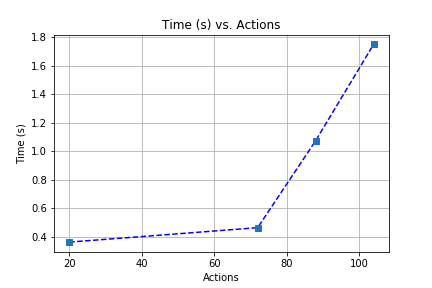
\includegraphics[width=1\columnwidth]{fig/results_131.png}
%\caption{Search Method GBFGS}
\end{center}
\caption{Greedy Best First Graph.}
\label{fig131}
\end{figure}

\begin{figure}[htpb]
\begin{center}
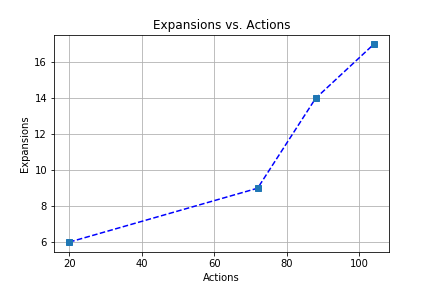
\includegraphics[width=1\columnwidth]{fig/results_134.png}
%\caption{Search Method GBFGS}
\end{center}
\caption{Greedy Best First Graph.}
\label{fig134}
\end{figure}

%\subsection{A* Search}
The A* search is the algorithm with the lesser number of expansions, as seen in Figure \ref{fig034}, and not much time in comparison with the others, Figure \ref{fig031}. Roughly, is possible to infer that this search algorithm is the best choice for this problem domain. This results is expected, because A* uses a better cost function, considering not only the cost to objective, but plus the cost from initial node to a possible expanded node. Considering the heuristics, for A* and GBFGS, it is possible to infer that Unmet Goals presents the better results: the search algorithm takes much less time and achieve good solutions (almost all optimal). 

\begin{figure}[htpb]
\begin{center}
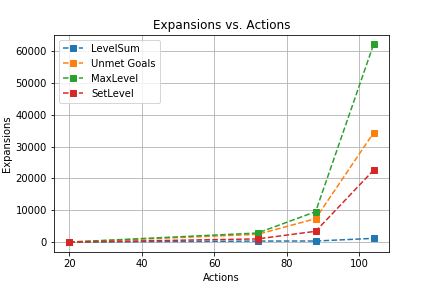
\includegraphics[width=1\columnwidth]{fig/results_034.png}
%\caption{Search Method AS}
\end{center}
\caption{A*.}
\label{fig034}
\end{figure}
        

%\subsection{A* Search}

\begin{figure}[htpb]
\begin{center}
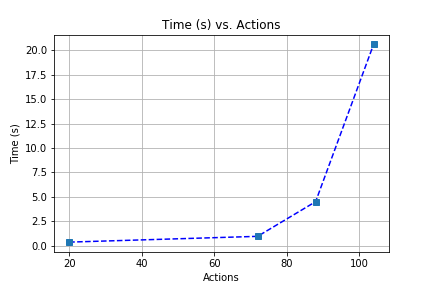
\includegraphics[width=1\columnwidth]{fig/results_031.png}
%\caption{Search Method AS}
\end{center}
\caption{A*.}
\label{fig031}
\end{figure}



In \cite{githubUdacityAINDProj2} is proposed to answer some questions about this work. 

\begin{itemize}
    \item Which algorithm or algorithms would be most appropriate for planning in a very restricted domain (i.e., one that has only a few actions) and needs to operate in real time?
    
    R: In this domain, with the problems formatted as shown, BFS, UCS and A* are good choices when we looking for optimal planning. In restricted domain, all of these algorithm takes a short time.
    
    \item Which algorithm or algorithms would be most appropriate for planning in very large domains (e.g., planning delivery routes for all UPS drivers in the U.S. on a given day)?
    
    R: The best choice may be A* with heuristic Unmet Goals, because this take a good relationship between time and quality of plan (optimal plan).
    
    \item Which algorithm or algorithms would be most appropriate for planning problems where it is important to find only optimal plans?
    
    UCS and BFS are the right choices, find the optimal solution in all problems. However, the A* with some good heuristic should be considered secondarily. 
    
\end{itemize}
    
\newpage

\section{Conclusion}

With this work, is possible to experiment some search algorithms and heuristics applying to a conceptual logistic problem. The different scales of the problem (different size of graphs) diversify the effects and results that, which shows the different characteristics between the search methods.

As expected,  the A* search algorithm presents the overall best results and, not so expected, the DFGS presents the wort results. Of course, only with these four search problems is it not possible to evaluate the methods in a general and conclusive way, but one can extract good experience and good notions from each one.


\bibliographystyle{IEEEtran}
\bibliography{bibliography.bib}

%\appendix
%\section{Jupyter Notebook: processing the results.}
%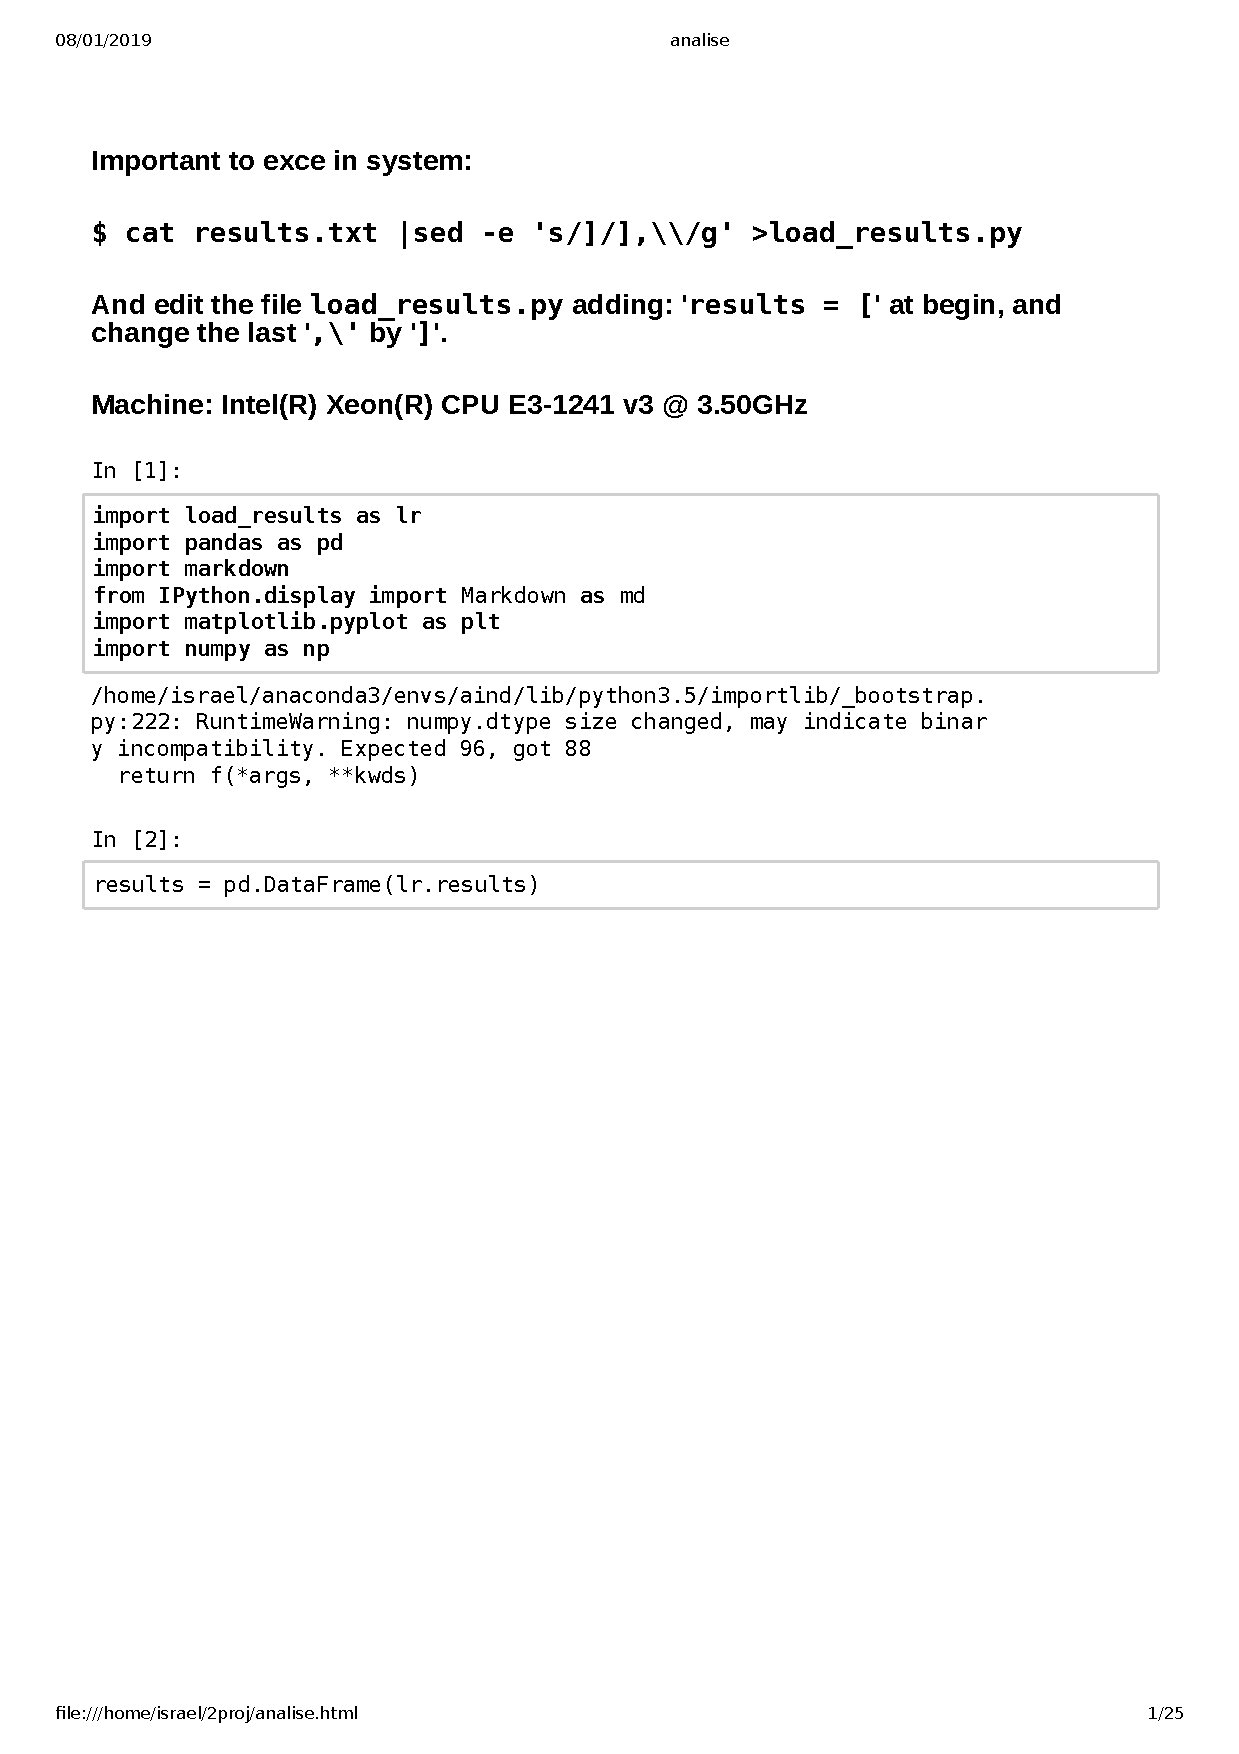
\includepdf{analise.pdf}

\end{document}